\documentclass[11pt]{article}
\usepackage{geometry}                % See geometry.pdf to learn the layout options. There are lots.
\geometry{letterpaper}                   % ... or a4paper or a5paper or ... 
\usepackage[parfill]{parskip}    % Activate to begin paragraphs with an empty line rather than an indent
\usepackage{graphicx}
\usepackage{amssymb}
\usepackage{epstopdf}

% matlab code
\usepackage[numbered]{mcode}
%\usepackage{listings}
%\lstset{language=matlab}

\lstset{float,frame=tb}
\lstdefinestyle{call}{numbers=none}

\title{Image Printing Based on Halftoning}
\author{Cody A. Ray}
%\date{}                                           % Activate to display a given date or no date

\begin{document}
\maketitle

\section{Project Goal}

This objective of this project was to develop an image printing program based on the concept of halftoning.\footnote{Due to differences in printer capabilities, half-tone images were written to file rather than printed.} The following figure shows ten shades of gray approximated by dot patterns.  Each gray level is represented by a 3~x~3 pattern of black and white dots.  A 3~x~3 area full of black dots is the approximation to gray-level black, or 0.  Similarly, a 3~x~3 area of white dots represents gray level 9, or white.  The other dot patterns are approximations to gray levels in between these two extremes.  A gray-level printing scheme based on dots patterns such as these is called  ``halftoning.''  Note that each pixel in an input image will correspond to 3~x~3 pixels on the printed image, so spatial resolution will be reduced to 33\% of the original in both the vertical and horizontal direction. 

\begin{figure}[ht]
   \centering
   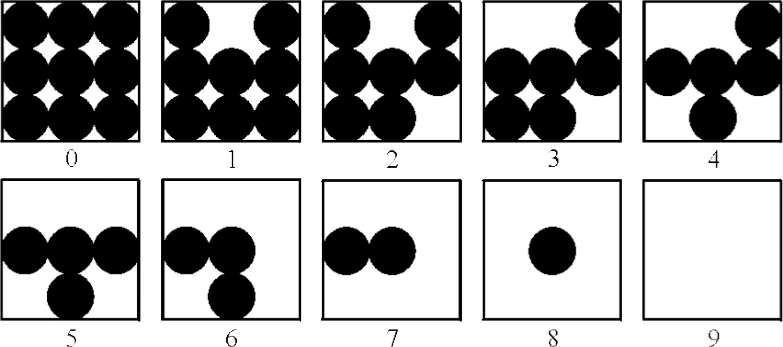
\includegraphics{halftone-dots.png}
   \caption{Halftone Dot Pattern Approximating Ten Shades of Gray}
   \label{fig:halftone-dots}
\end{figure}

\section{Findings and Conclusions}

This halftoning specification, containing only ten shades of gray and having the dots evenly spaced and sized, leaves much to be desired in the quality of the halftoned image. While this specification was simple to implement and has reasonable runtime performance,  there are a few clear disadvantages. The multidimensional reduction in spatial resolution is clearly unacceptable, resulting in a very low-quality halftoned image. Furthermore, the resulting three-fold increase in size creates logistical difficulties in scaling images for various applications (e.g., printing, word processing, etc). The disadvantages definitely outweigh the advantages, and this halftoning specification is not recommended to be used.

\section{Supporting Data}
\label{sec:data}

The system was implemented in MATLAB and tested with images that came with the textbook or were pre-installed with MATLAB.

To ensure the logic was correctly implemented, the first test conducted was with a matrix rather than an actual image. Listing~\ref{lst:halftonetest} shows the input image \texttt{in\_img}, the image after scaling to the full grayscale range \texttt{mid\_img}, and the resulting halftone image \texttt{out\_img}. In this halftone matrix, each pixel is replaced by the corresponding set of black and white dots, where a black dot is represented by 0 and a white dot by 1.

\begin{lstlisting}[style=call,label=lst:halftonetest,caption={Testing the Halftoning System}]
in_img =

     1     2     3
     4     5     6
     7     8     9


mid_img =

     0     1     2
     3     5     6
     7     8     9


out_img =

     0     0     0     0     1     0     0     1     0
     0     0     0     0     0     0     0     0     0
     0     0     0     0     0     0     0     0     1
     1     1     0     1     1     1     1     1     1
     0     0     0     0     0     0     0     0     1
     0     0     1     1     0     1     1     0     1
     1     1     1     1     1     1     1     1     1
     0     0     1     1     0     1     1     1     1
     1     1     1     1     1     1     1     1     1
\end{lstlisting}

A visual comparison of \texttt{out\_img} and \texttt{mid\_img} to the dot configurations in Fig.~\ref{fig:halftone-dots} shows that the system is implemented correctly per specification.

The first image with which the program was tested was the football photograph bundled with MATLAB. However, as the program only accepts monochromatic images, the photograph was first converted to grayscale with the command \texttt{rgb2gray}. For this report, the original image was scaled using photoshop prior to halftone processing so that the halftoned image (which is three times as large) can fit on the page. The original (unscaled) image appears in Fig.~\ref{fig:football}, and the halftoned image is shown in Fig.~\ref{fig:football-halftone}.

\begin{figure}[ht]
   \centering
   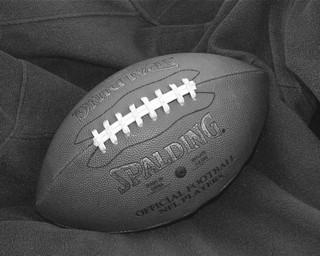
\includegraphics{../../imgin/football.jpg}
   \caption{Original Football Image (Unscaled)}
   \label{fig:football}
\end{figure}

\begin{figure}[ht]
   \centering
   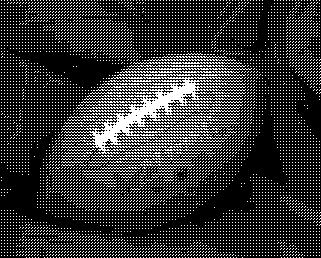
\includegraphics{../../imgout/halftone-football33per.jpg}
   \caption{Halftoned Football Image}
   \label{fig:football-halftone}
\end{figure}

The second image tested was the near-famous image of ``Lena'' distributed with the textbook \textit{Digital Image Processing} by Gonzales and Woods. The note from above regarding scaling for the report applies to this image as well. Additionally, the image was first converted from BMP format to JPG format using the ImageMagick \texttt{convert} command.

\begin{figure}[ht]
   \centering
   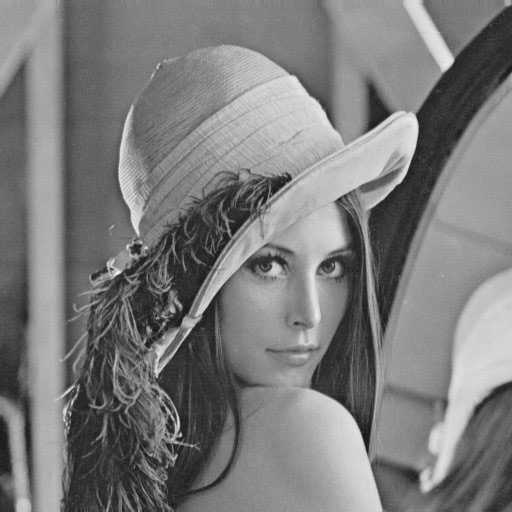
\includegraphics[scale=.4]{lena.jpg}
   \caption{Original Lena Image (Scaled)}
   \label{fig:lena}
\end{figure}

\begin{figure}[ht]
   \centering
   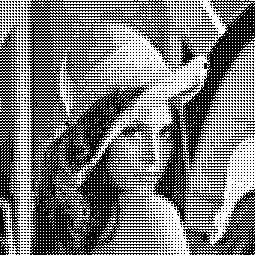
\includegraphics{halftone-lena33per50per.jpg}
   \caption{Halftoned Lena Image}
   \label{fig:lena-halftone}
\end{figure}

\clearpage
\appendix
\section{Computer Programs}

\lstinputlisting[label=lst:halftone,caption={Source Code of halftone.m}]{../../src/halftone.m}

\newpage
\lstinputlisting[label=lst:usage,caption={Source Code of usage.m}]{../../src/usage.m}

\end{document}  